\documentclass[a4paper,twoside,BCOR=20mm]{scrreprt}
\usepackage[utf8]{inputenc}
\usepackage[T1]{fontenc}
\usepackage[ngerman]{babel}	% german hyphenation, quotes, etc
\usepackage[ngerman]{translator}
\usepackage{amsmath}
\usepackage{paralist}
\usepackage{amsfonts}
\usepackage{acronym}
\usepackage{enumerate}
\usepackage{hyperref}
\usepackage{amssymb}
\usepackage{caption}
\usepackage{multirow}
\usepackage{graphicx}
\usepackage{tabularx}
\usepackage{color}
\usepackage{wrapfig} % wrap text around figures
\usepackage{subfig} % align two pics beside each other
\usepackage[table,xcdraw]{xcolor}
\hypersetup{ 					% ‘texdoc hyperref‘ for options
	pdftitle={PSE PCC: Designentwurf},
	pdfauthor={Giorgio Groß, Christoph Hörtnagl, David Laubenstein,  Josh Romanowski,  Fabian Wenzel},
	bookmarks=true,
}
\title{Designentwurf: Privacy Crash- Cam}

%Paket laden
\usepackage[
numberedsection,
nonumberlist, %keine Seitenzahlen anzeigen
acronym,      %ein Abkürzungsverzeichnis erstellen
toc,          %Einträge im Inhaltsverzeichnis
section]      %im Inhaltsverzeichnis auf section-Ebene erscheinen
{glossaries}

%Befehle für Abkürzungen
\newacronym{KIT}{KIT}{Karlsruher Institut für Technologie}

%Richtige Silbentrennungen
\hyphenation{Ein-stel-lun-gen}

% KIT layout

\definecolor{orange}{rgb}{1,0.5,0}
\definecolor{mintgreen}{RGB}{50,161,137}
\definecolor{gray}{RGB}{120,120,120}

\usepackage[color]{changebar}
\cbcolor{gray}
\changebarwidth 0.5pt

\usepackage{fancyhdr}
\pagestyle{fancy}
 \fancyhf{} %alle Kopf- und Fußzeilenfelder bereinigen 
 
 \fancypagestyle{plain}{} %Kopf- und Fußzeile auf jeder Seite	 
	\fancyhead[L]{PCC-Designentwurf}
	\fancyhead[R]{\leftmark}
	\rhead{\nouppercase{\leftmark}}
	\renewcommand{\headrulewidth}{0.5pt}
	\renewcommand{\headrule}{\hbox to\headwidth{%
		\color{mintgreen}\leaders\hrule height \headrulewidth\hfill}}

\raggedbottom

	\renewcommand{\footrulewidth}{0.5pt}
	\renewcommand{\footrule}{\hbox to\headwidth{%
  		\color{mintgreen}\leaders\hrule height \headrulewidth\hfill}}				
	\fancyfoot[LE,RO]{\thepage}


\setcounter{tocdepth}{5}
\makeglossaries
\begin{document}
\begin{titlepage}

\begin{center}


\includegraphics[width=0.5\linewidth]{Res/KITLogo.png}\\[0.5cm]
  

\textsc{\bfseries Fraunhofer Institut für Optronik, Systemtechnik und Bildauswertung}\\[0.5cm]
\textsc{Mario Kaufmann\\Pascal Birnstill\\Erik Krempel}\\[2cm]

\textsc{\LARGE \bfseries Designentwurf}\\[0.5cm]
\textsc{\bfseries Version 0.1}\\[0.2cm]


\newcommand{\HRule}{\rule{\linewidth}{0.5mm}} 
{\color{mintgreen}\HRule} \\[0.4cm]
{\huge \bfseries Privacy Crash Cam App für Android}\\[0.4cm]
{\color{mintgreen}\HRule} \\[1cm]

% \textsc{\Large \bfseries Gruppe :}\\[0.3cm] 
\textsc{\Large Fabian Wenzel\\ Giorgio Groß\\ Christoph Hörtnagl\\ David Laubenstein\\[0.15cm]Josh Romanowski} \\[2cm]

{\large \today}

\end{center}

\end{titlepage}
% \maketitle
\tableofcontents
\newpage
%content
\include{./subtopicsDesign/Zielbestimmung}
\chapter{Anhang}

\section{Sequenzdiagramme}

\begin{figure}[ht]
	\centering
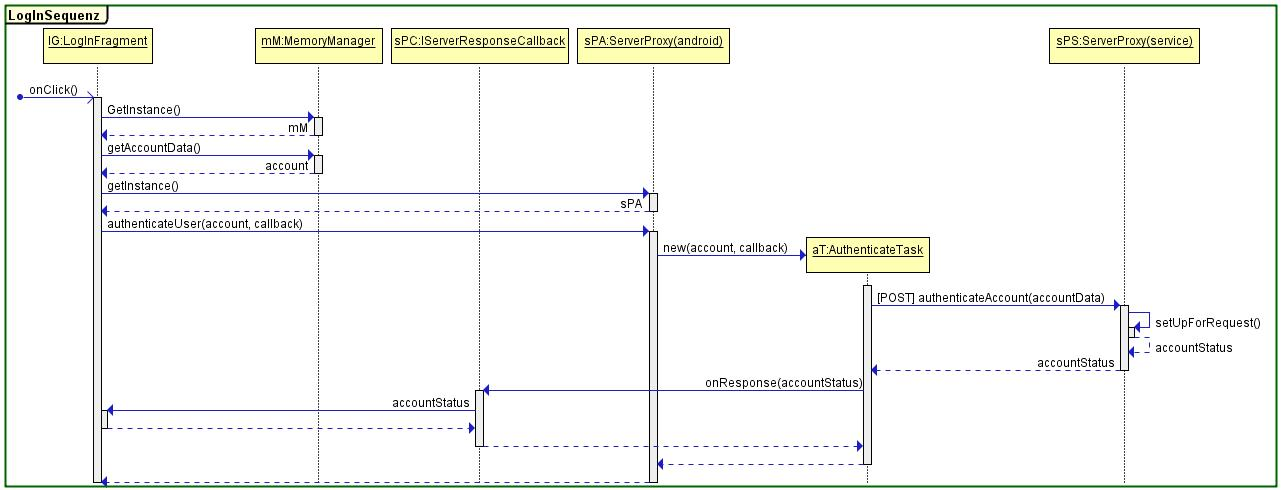
\includegraphics[width=1\textwidth]{./resources/Diagramme/App/logInSequence.jpg}
\caption{Anmelden in der App}
	\label{fig:AppAuth}
\end{figure}

\begin{figure}[ht]
	\centering
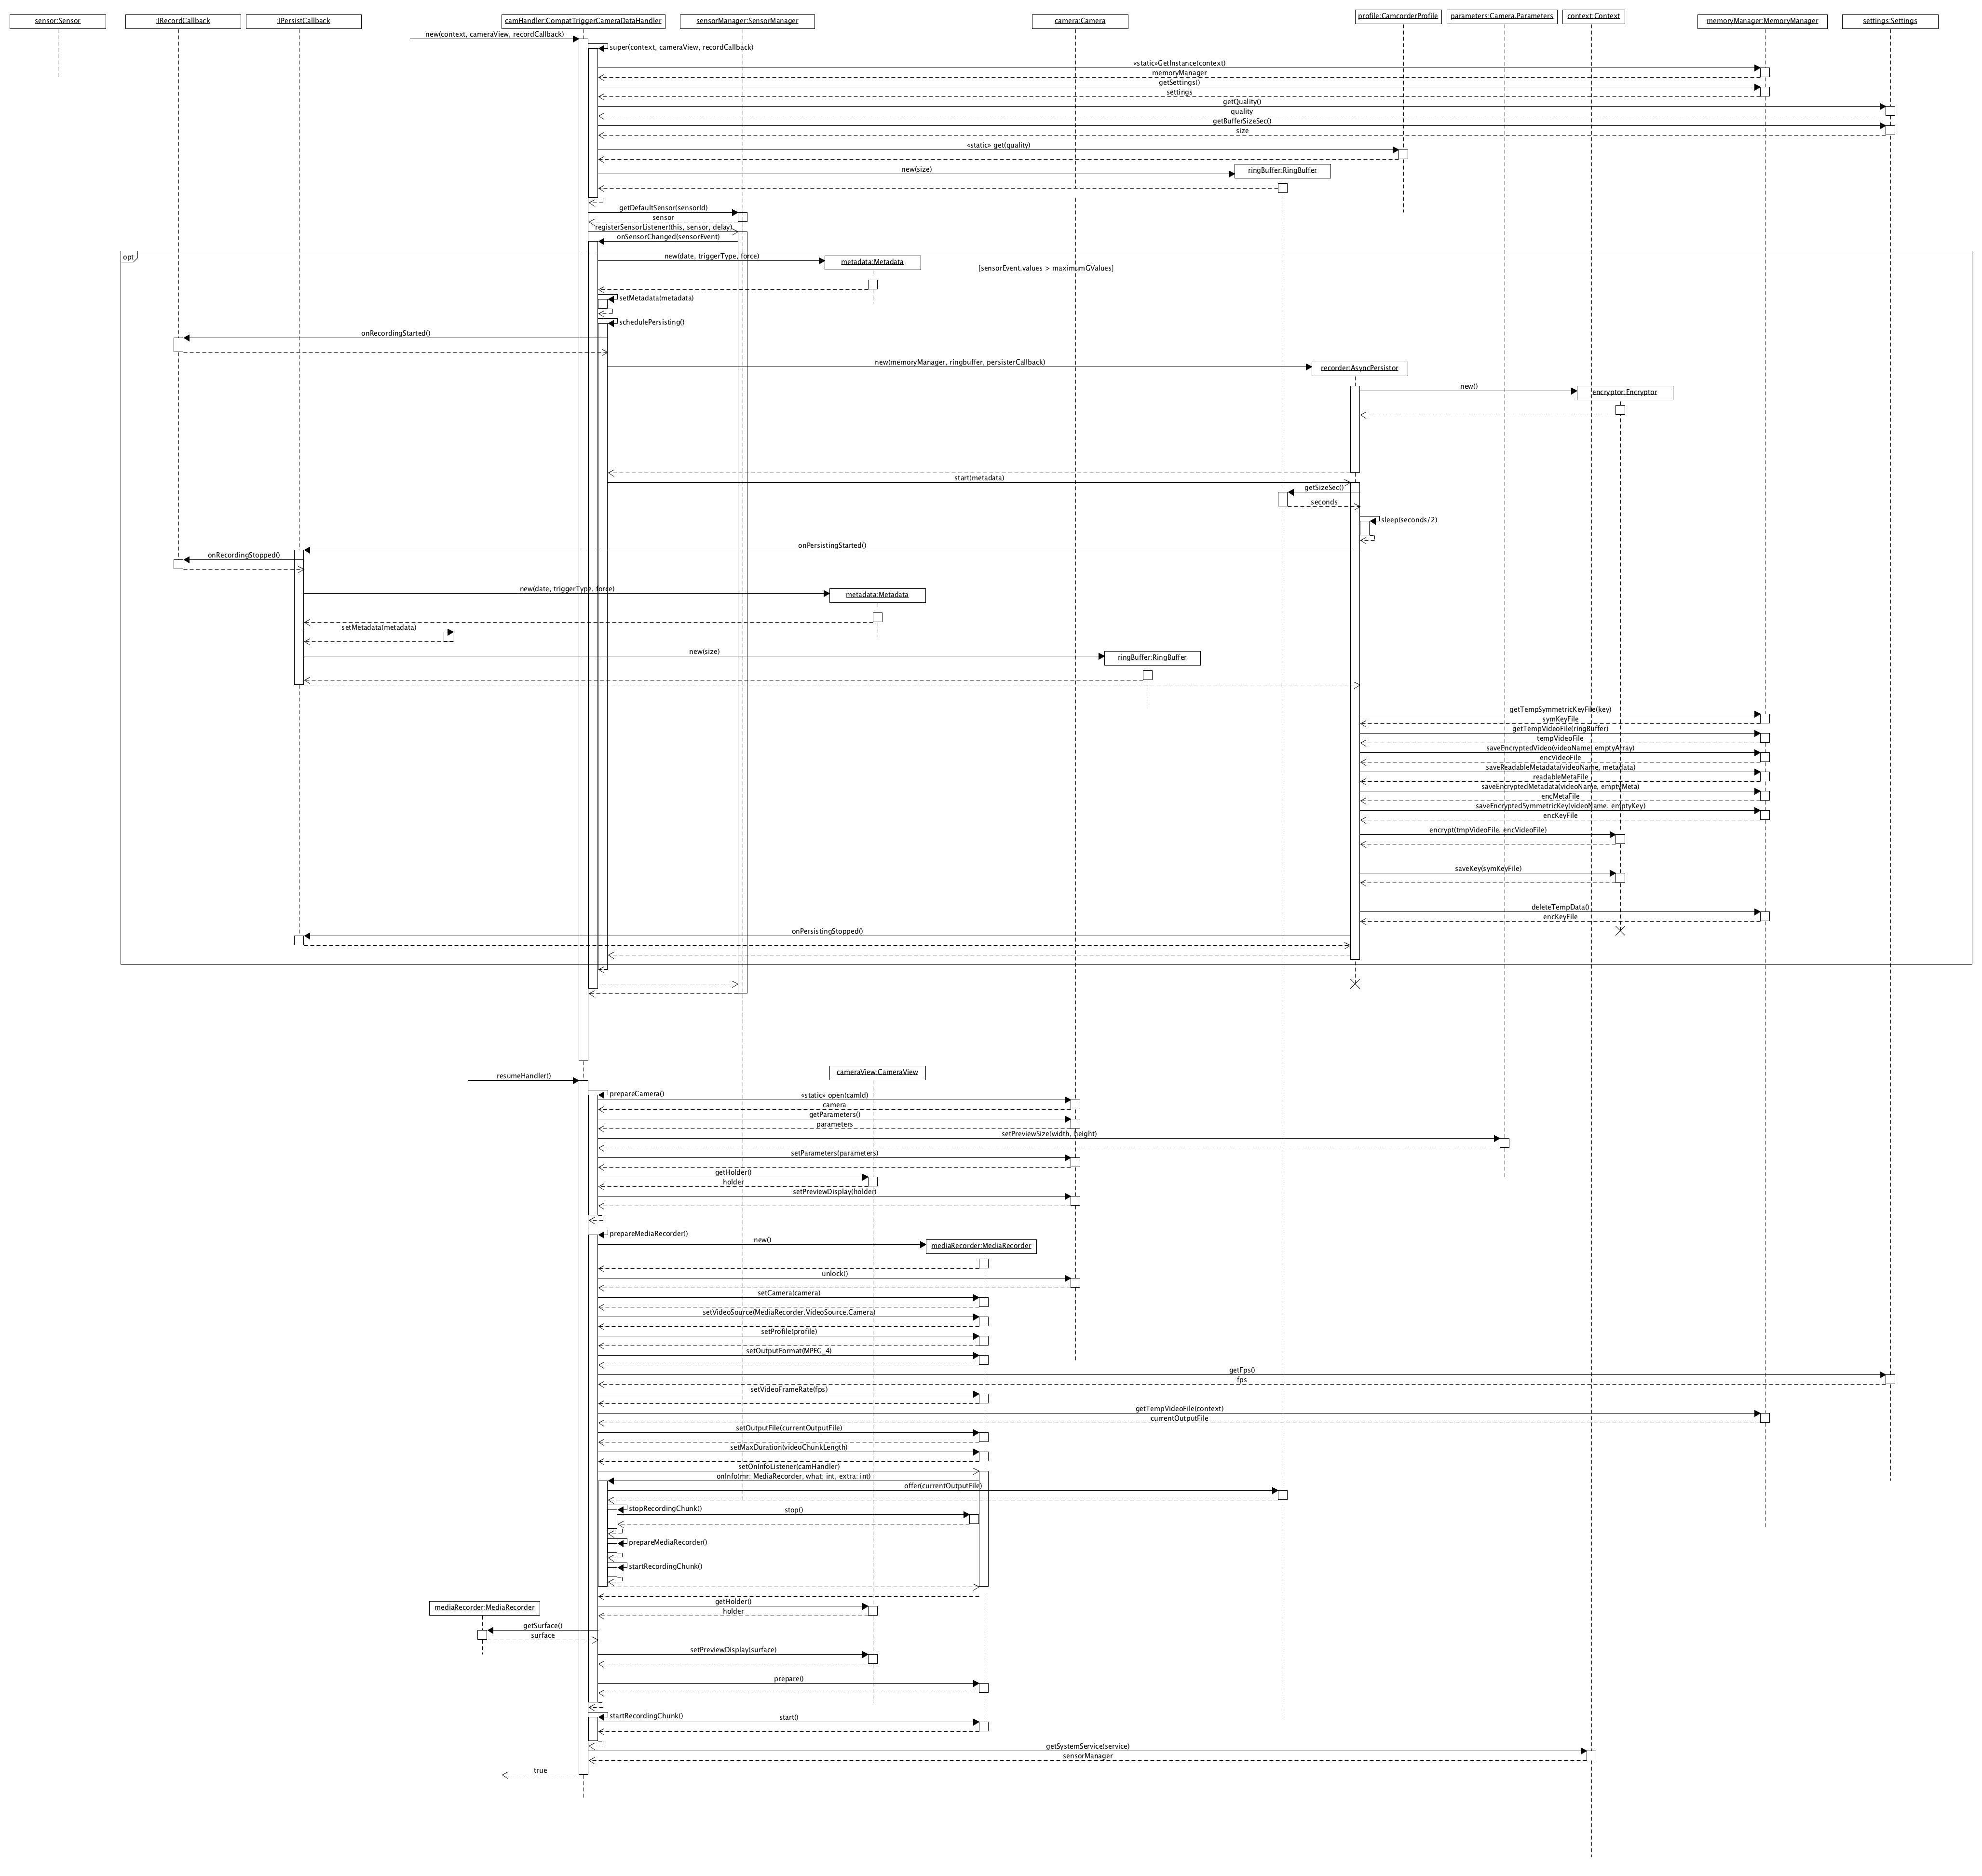
\includegraphics[width=1\textwidth]{./resources/Diagramme/App/recordSequence.jpg}
\caption{Videoaufnahme in der App}
	\label{fig:AppVideo}
\end{figure}

\begin{figure}[ht]
	\centering
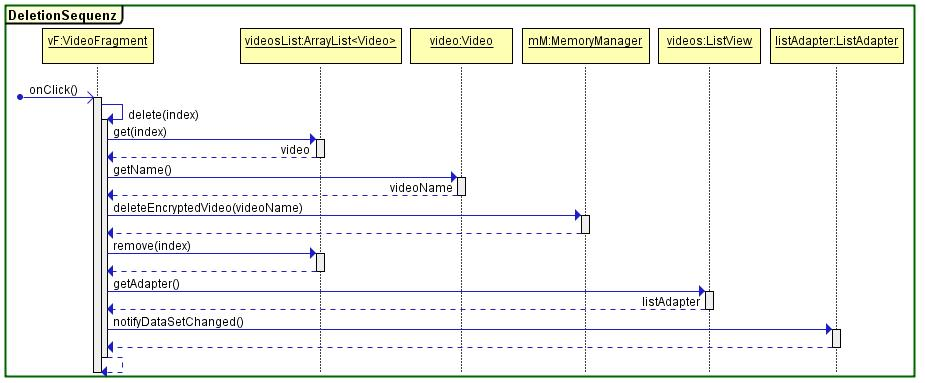
\includegraphics[width=1\textwidth]{./resources/Diagramme/App/deleteVideoSequence.jpg}
\caption{Video in der App löschen}
	\label{fig:AppDel}
\end{figure}

\begin{figure}[ht]
	\centering
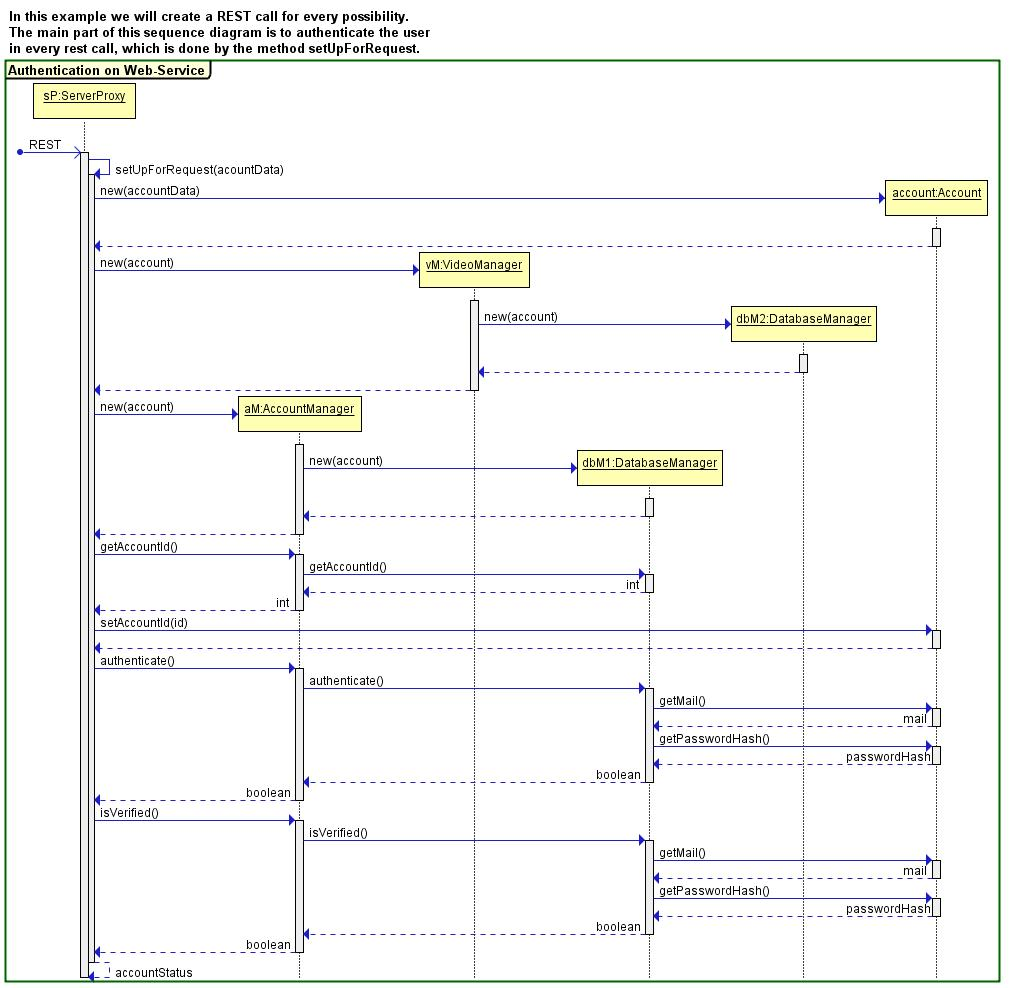
\includegraphics[width=1\textwidth]{./resources/Diagramme/Webservice/SeqAuthenticate.jpg}
\caption{Authentifizieren auf dem Dienst}
	\label{fig:ServiceAuth}
\end{figure}

\begin{figure}[ht]
	\centering
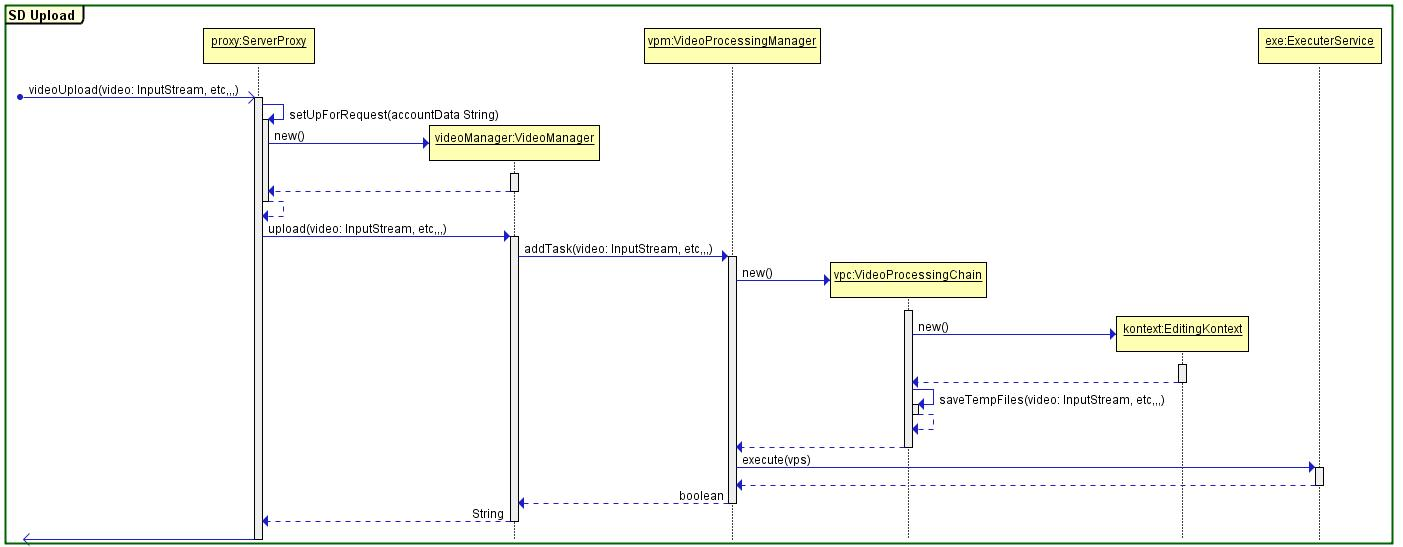
\includegraphics[width=1\textwidth]{./resources/Diagramme/Webservice/Upload.jpg}
\caption{Video auf den Dienst hochladen}
	\label{fig:ServiceUpload}
\end{figure}

\begin{figure}[ht]
	\centering
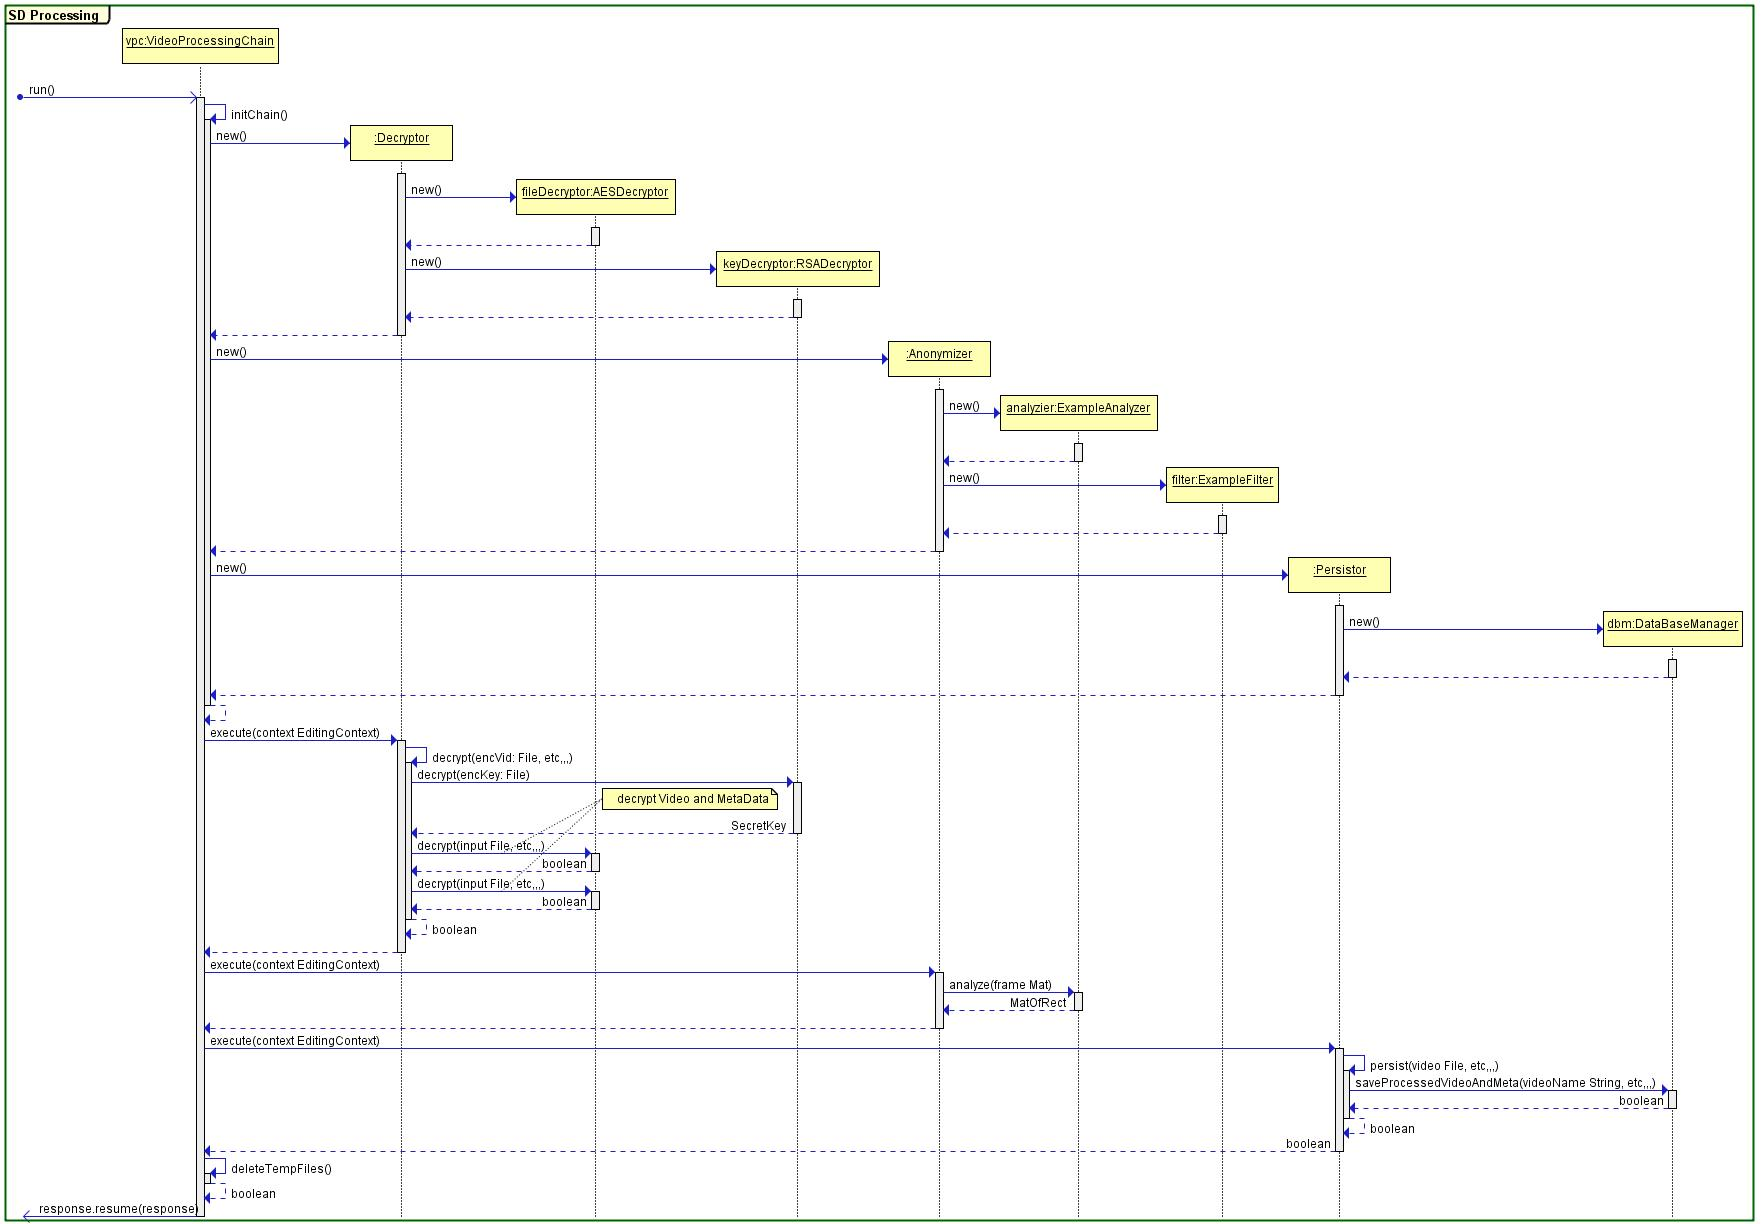
\includegraphics[width=1\textwidth]{./resources/Diagramme/Webservice/Processing.jpg}
\caption{Videobearbeitung auf dem Dienst}
	\label{fig:ServiceProcess}
\end{figure}

\begin{figure}[ht]
	\centering
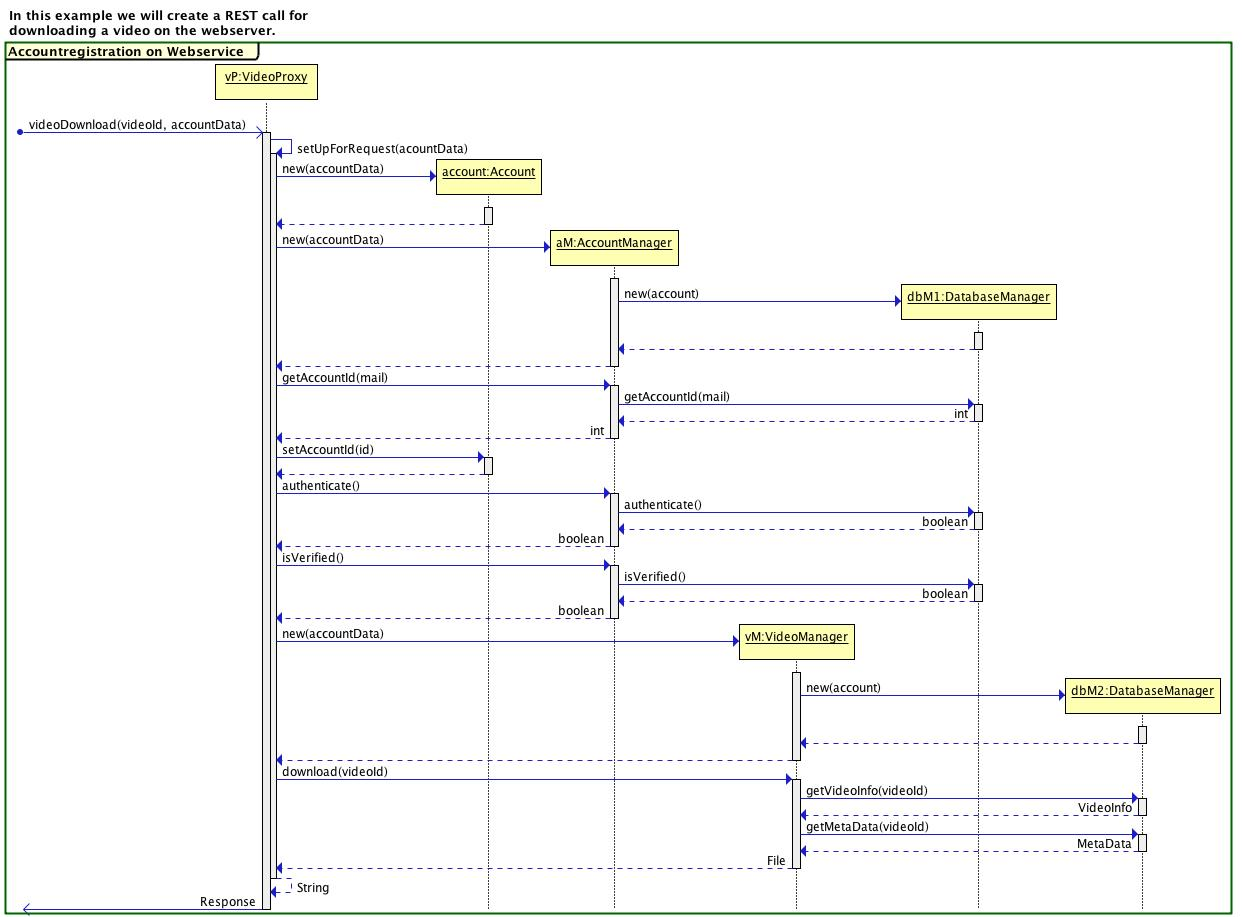
\includegraphics[width=1\textwidth]{./resources/Diagramme/Webservice/SeqVideoDownload.jpg}
\caption{Videodownload vom Dienst}
	\label{fig:ServiceDownl}
\end{figure}

\begin{figure}[ht]
	\centering
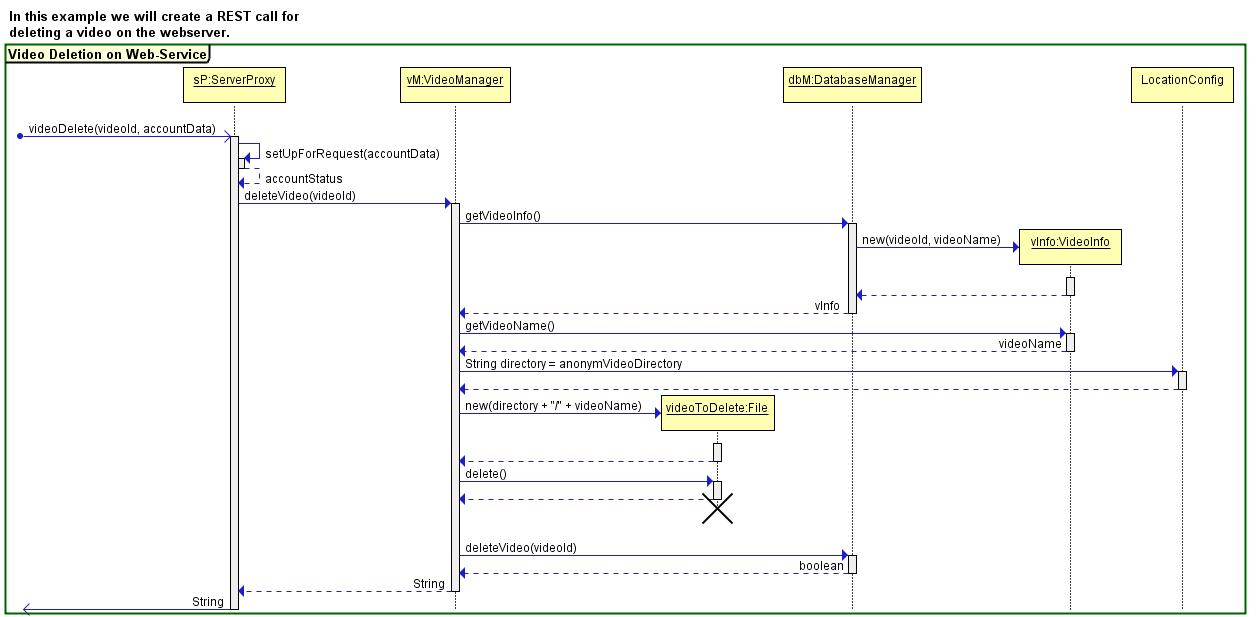
\includegraphics[width=1\textwidth]{./resources/Diagramme/Webservice/SeqVideoDeletion.jpg}
\caption{Video auf dem Dienst löschen}
	\label{fig:ServiceDel}
\end{figure}
%end content

\end{document}

